\documentclass[border=3pt]{standalone}
% Preâmbulo compartilhado pelos diagramas TikZ da aula 8 de IHC (Design de IHC)
\usepackage[T1]{fontenc}
\usepackage[utf8]{inputenc}
\usepackage{lmodern}
\usepackage{amsmath}
\usepackage{xcolor}
\usepackage{tikz}
\usetikzlibrary{arrows.meta,angles,quotes,decorations.pathmorphing,decorations.pathreplacing,calc,
                positioning,shapes.geometric,shapes.misc,backgrounds,fit,
                math}

% Paleta (mesma dos SVGs originais)
% Paleta da disciplina de IHC: acento roxo (#755099), da capa do livro.
% (o nome "dblue" é mantido para não alterar todos os diagramas)
\definecolor{dblue}{HTML}{755099}
\definecolor{dorange}{HTML}{B3541E}
\definecolor{dgreen}{HTML}{4A7C59}
\definecolor{dred}{HTML}{9C4B4B}
\definecolor{dcream}{HTML}{F4F1EA}
\definecolor{dshade}{HTML}{DDD7C9}

% Função gaussiana (não normalizada por padrão de escala visual)
\pgfmathdeclarefunction{gauss}{3}{%
  \pgfmathparse{1/(#3*sqrt(2*pi))*exp(-((#1-#2)^2)/(2*#3^2))}%
}

% Estilos comuns (prefixo d... para não colidir com chaves internas do pgf)
\tikzset{
  >={Stealth[length=2mm]},
  dguide/.style={gray!55, dashed, line width=0.4pt},
  daxis/.style={gray!60, line width=0.7pt, ->},
  dbody/.style={fill=black!3, draw=black!80, line width=1pt},
  dacc/.style={draw=dblue, line width=1pt},
  dlbl/.style={black!55, font=\small},
  dsub/.style={black!45, font=\footnotesize},
  dstate/.style={circle, draw=black!80, fill=dcream, line width=1pt,
                 minimum size=17mm, font=\large, inner sep=1pt},
  dobs/.style={circle, draw=black!80, fill=dshade, line width=1pt,
               minimum size=14mm, font=\large, inner sep=1pt},
  dbox/.style={rounded corners=2pt, draw=black!80, fill=dcream, line width=1pt,
               align=center, inner sep=6pt},
  dop/.style={circle, draw=black!80, fill=white, line width=1pt,
              minimum size=6mm, inner sep=0pt, font=\small},
  dtrans/.style={->, dblue, line width=1pt},
  dmeas/.style={->, dorange, line width=1pt},
  dcurve/.style={line width=1pt, dblue},
  dcurveb/.style={line width=1.4pt, dorange},
}

\begin{document}
\hyphenpenalty=10000 \exhyphenpenalty=10000 \tolerance=9999 \emergencystretch=3em
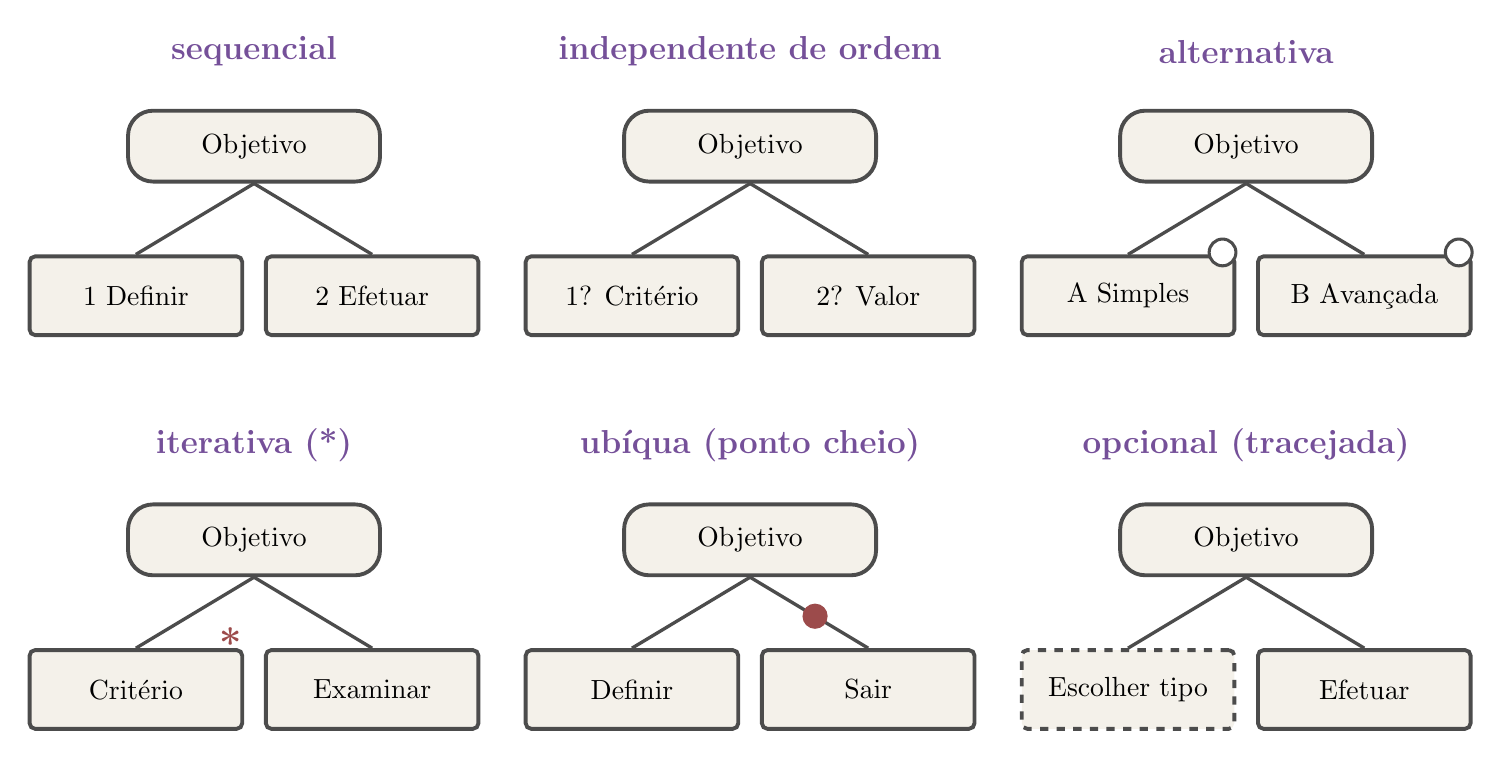
\begin{tikzpicture}[x=1cm,y=1cm]
\node[font=\large\bfseries, dblue] at (3.2,8.7) {sequencial};
\node[dbox, draw=black!70, rounded corners=9pt, line width=1.4pt, minimum width=3.2cm, minimum height=0.9cm, font=\normalsize] (p) at (3.2,7.5) {Objetivo};
\node[dbox, draw=black!70, line width=1.4pt, minimum width=2.7cm, minimum height=1.0cm, font=\normalsize, inner sep=3pt] (k0) at (1.7000000000000002,5.6) {1 Definir};
\draw[black!70, line width=1.2pt] (p.south) -- (k0.north);
\node[dbox, draw=black!70, line width=1.4pt, minimum width=2.7cm, minimum height=1.0cm, font=\normalsize, inner sep=3pt] (k1) at (4.7,5.6) {2 Efetuar};
\draw[black!70, line width=1.2pt] (p.south) -- (k1.north);
\node[font=\large\bfseries, dblue] at (9.5,8.7) {independente de ordem};
\node[dbox, draw=black!70, rounded corners=9pt, line width=1.4pt, minimum width=3.2cm, minimum height=0.9cm, font=\normalsize] (p) at (9.5,7.5) {Objetivo};
\node[dbox, draw=black!70, line width=1.4pt, minimum width=2.7cm, minimum height=1.0cm, font=\normalsize, inner sep=3pt] (k0) at (8.0,5.6) {1? Critério};
\draw[black!70, line width=1.2pt] (p.south) -- (k0.north);
\node[dbox, draw=black!70, line width=1.4pt, minimum width=2.7cm, minimum height=1.0cm, font=\normalsize, inner sep=3pt] (k1) at (11.0,5.6) {2? Valor};
\draw[black!70, line width=1.2pt] (p.south) -- (k1.north);
\node[font=\large\bfseries, dblue] at (15.8,8.7) {alternativa};
\node[dbox, draw=black!70, rounded corners=9pt, line width=1.4pt, minimum width=3.2cm, minimum height=0.9cm, font=\normalsize] (p) at (15.8,7.5) {Objetivo};
\node[dbox, draw=black!70, line width=1.4pt, minimum width=2.7cm, minimum height=1.0cm, font=\normalsize, inner sep=3pt] (k0) at (14.3,5.6) {A Simples};
\draw[black!70, line width=1.2pt] (p.south) -- (k0.north);
\node[dbox, draw=black!70, line width=1.4pt, minimum width=2.7cm, minimum height=1.0cm, font=\normalsize, inner sep=3pt] (k1) at (17.3,5.6) {B Avançada};
\draw[black!70, line width=1.2pt] (p.south) -- (k1.north);
\draw[black!70, fill=white, line width=1.1pt] (15.5,6.1499999999999995) circle (0.17);
\draw[black!70, fill=white, line width=1.1pt] (18.5,6.1499999999999995) circle (0.17);
\node[font=\large\bfseries, dblue] at (3.2,3.7) {iterativa (*)};
\node[dbox, draw=black!70, rounded corners=9pt, line width=1.4pt, minimum width=3.2cm, minimum height=0.9cm, font=\normalsize] (p) at (3.2,2.5) {Objetivo};
\node[dbox, draw=black!70, line width=1.4pt, minimum width=2.7cm, minimum height=1.0cm, font=\normalsize, inner sep=3pt] (k0) at (1.7000000000000002,0.6) {Critério};
\draw[black!70, line width=1.2pt] (p.south) -- (k0.north);
\node[dbox, draw=black!70, line width=1.4pt, minimum width=2.7cm, minimum height=1.0cm, font=\normalsize, inner sep=3pt] (k1) at (4.7,0.6) {Examinar};
\draw[black!70, line width=1.2pt] (p.south) -- (k1.north);
\node[font=\Large\bfseries, dred] at (2.9000000000000004,1.2) {*};
\node[font=\large\bfseries, dblue] at (9.5,3.7) {ubíqua (ponto cheio)};
\node[dbox, draw=black!70, rounded corners=9pt, line width=1.4pt, minimum width=3.2cm, minimum height=0.9cm, font=\normalsize] (p) at (9.5,2.5) {Objetivo};
\node[dbox, draw=black!70, line width=1.4pt, minimum width=2.7cm, minimum height=1.0cm, font=\normalsize, inner sep=3pt] (k0) at (8.0,0.6) {Definir};
\draw[black!70, line width=1.2pt] (p.south) -- (k0.north);
\node[dbox, draw=black!70, line width=1.4pt, minimum width=2.7cm, minimum height=1.0cm, font=\normalsize, inner sep=3pt] (k1) at (11.0,0.6) {Sair};
\draw[black!70, line width=1.2pt] (p.south) -- (k1.north);
\fill[dred] ($(p.south)!0.55!(k1.north)$) circle (0.16);
\node[font=\large\bfseries, dblue] at (15.8,3.7) {opcional (tracejada)};
\node[dbox, draw=black!70, rounded corners=9pt, line width=1.4pt, minimum width=3.2cm, minimum height=0.9cm, font=\normalsize] (p) at (15.8,2.5) {Objetivo};
\node[dbox, draw=black!70, dashed, line width=1.4pt, minimum width=2.7cm, minimum height=1.0cm, font=\normalsize, inner sep=3pt] (k0) at (14.3,0.6) {Escolher tipo};
\draw[black!70, line width=1.2pt] (p.south) -- (k0.north);
\node[dbox, draw=black!70, line width=1.4pt, minimum width=2.7cm, minimum height=1.0cm, font=\normalsize, inner sep=3pt] (k1) at (17.3,0.6) {Efetuar};
\draw[black!70, line width=1.2pt] (p.south) -- (k1.north);
\end{tikzpicture}
\end{document}
